\chapter{Kvantno računalo}

\section{Polarizacija svjetlosti}

Klasična fizika shvaća svjetlost kao transverzalni elektromagnetski val koji može biti poraliziran na različite načine. Polarizacija svjetlosti određena je njenom električnom komponentom te je svjetlost koju emitiraju prirodni izvori svjetlosti uglavnom nepolarizirana. Tek kada se snop svjetlosti pusti kroz polarizator dobije se linearno polariziran val svjetlosti --- val koji ima stalni smjer širenja okomit na smjer titranja. Njegova električna komponenta dana je jednadžbom:
\begin{equation}
E = E_0 \hat{p}e^{i\omega t}
\end{equation}
gdje je $\hat{p}$ jedinični vektor u smjeru polarizacije vala. Intenzitet ovako polariziranog vala biti će upola manji od intenziteta početnog nepolariziranog vala jer će točno toliko intenziteta polarizator apsorbirati. Kada ovakav val pustimo kroz još jedan polarizator (tzv. analizator), val koji ćemo dobiti jest:
\begin{equation}
E' = (E \cdot \hat{n}) \hat{n} = E_0 (\hat{p} \cdot \hat{n})\hat{n}e^{i\omega t} = E_0 \cos \alpha
\end{equation}
gdje je $\hat{n}$ jedinični vektor u smjeru polarizacije analizatora, a $\alpha$ kut između vektora $\hat{p}$ i $\hat{n}$. Intenzitet novog vala dobivamo po Malusovom zakonu:
\begin{equation}
I' = I \cos^2 \alpha
\end{equation}
gdje je $I$ intenzitet prethodno polariziranog vala. Drugim riječima, polarizacijom vala dobivamo njegovu projekciju na ravninu određenu kutom polarizatora. 

U kvantnoj mehanici, svjetlost je definirana drugačije --- kao niz fotona, nedjeljivih elementarnih čestica. Kod takve interpretacije postavlja se pitanje što se događa kada individualni fotoni prolaze kroz polarizator. Ako polarizator propušta projekciju, koja je uvijek manja ili jednaka ulaznom valu, što će se dogoditi fotonu, ako je on nedjeljiv? Eksperimenti su pokazali da će foton sa točno određenom šansom ili cijeli proći kroz polarizator sa novim smjerom polarizacije ili biti apsorbiran. Ključan element takvih eksperimenata je činjenica da je nemoguće \emph{niti u načelu} odrediti što će se dogoditi sa fotonom. To znači da čak uz poznavanje svih varijabli nekog sustava, nemoguće je deterministički odrediti ishod.

Prijelaze kvantnih sustava iz jednog stanja u drugo modeliramo takozvanom amplitudom vjerojatnosti:
\begin{equation}
a(\phi \rightarrow \psi)
\end{equation}
koja je element skupa kompleksnih brojeva, a vjerojatnost da neki sustav koji je u stanju $\phi$ bude izmjeren u stanju $\psi$ dobivamo na način:
\begin{equation}
p(\phi \rightarrow \psi) = |a(\phi \rightarrow \psi)|^2
\end{equation}

U slučaju polarizatora, vjerojatnost smo mogli izračunati pomoću Malusovog zakona što nam daje vjerojatnost prolaska fotona kroz polarizator jednaku
\begin{equation}
p(\phi \rightarrow \psi) = \cos^2 \alpha
\end{equation}
iz čega je vidljiva amplituda vjerojatnosti:
\begin{equation}
|a(\phi \rightarrow \psi)|^2 = \cos^2 \alpha \Rightarrow a(\phi \rightarrow \psi) = \cos \alpha
\end{equation}
gdje je $\alpha$ kut koji zatvaraju vektori polarizacije fotona i polarizatora, $\phi$ stanje fotona prije prolaska kroz polarizator, a $\psi$ stanje u kojemu foton nije apsorbiran.

%Sličan primjer polarizatoru je dvolomac koji također funkcionira kao polarizator, samo što ne apsorbira svjetlost, nego dijeli svjetlost na dva ortogonalno polarizirana snopa. Koristeći dvolomac moguće je pomoću dva detektora izmjeriti u kojem je točno stanju foton završio. Nakon mjerenja, tj. detekcije, foton je apsorbiran.


\section{Kvantni bit}

\subsection{Svojstva}
Umjesto polarizatora moguće je koristiti i dvolomac koji također funkcionira kao polarizator, samo što ne apsorbira dio svjetlosti, nego dijeli svjetlost na dva ortagonalno polarizirana snopa. Kombinirajući dvolomac sa dva detektora fotona uvijek je moguće odrediti u koje je stanje prešao foton.
\begin{figure}[h!]
\centering
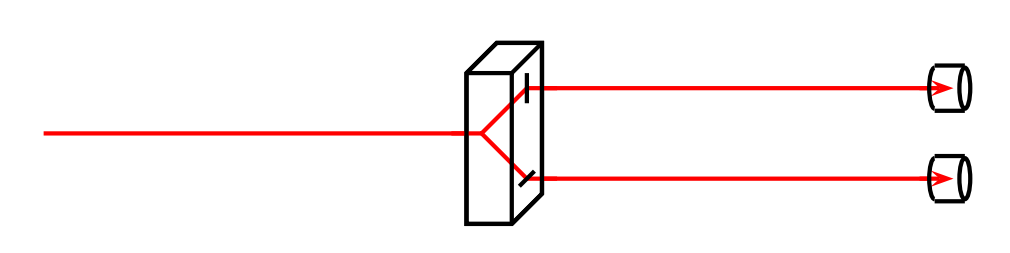
\includegraphics[scale=0.5]{img/dvolomac_detektor.png}
\caption{Dvolomac s dva detektora} 
\end{figure}

Nakon detekcije, foton je apsorbiran i ne može se više mjeriti. Takav kvantnomehanički sustav, koji je moguće samo jednom izmjeriti u samo jednom od dva moguća stanja nazivamo \textbf{kvantnim bitom} ili \textbf{qubitom}.
Kvantni bit prije mjerenja može biti u beskonačno mnogo različitih stanja te općenito jedno takvo stanje zovemo \textbf{superpozicijom} dvaju stanja. Ta dva stanja se odnose na stanja baze koja mogu biti proizvoljna, ali su uvijek međusobno ortogonalna. Pojam superpozicije se može primijeniti i u klasičnom smislu. U slučaju svjetlosti, uzimajući dva linearno polarizirana vala s okomitim smjerovima polarizacije kao bazu sustava, općenito stanje polarizacije vala možemo prikazati kao:
\begin{equation}
E = E_x \hat{x}e^{i(\omega t + \phi_x)} + E_y \hat{y}e^{i(\omega t + \phi_y)} = E_0(\lambda \hat{x} + \mu \hat{y})e^{i\omega t}
\end{equation}
gdje vrijedi:
\begin{equation}
E_0 = \sqrt{(E_x^2 + E_y^2)}
\qquad
\lambda = \frac{E_x}{E_0}e^{i\phi_x}
\qquad
\mu = \frac{E_y}{E_0}e^{i\phi_y}
\qquad
|\lambda|^2 + |\mu|^2 = 1
\end{equation}
Bitno je uočiti da su $\lambda$ i $\mu$ kompleksni brojevi kao i da dio izraza $\lambda\hat{x}+\mu\hat{y}$ sadrži informaciju o stanju polarizacije vala te da takvih stanja ima beskonačno mnogo.

\subsection{Diracova notacija}

% DIRACOVA NOTACIJA i sva pravila - Hilbertov prostor itd
% izracunati vjerojatnost
% vektorski prikaz

\subsection{Prikaz na klasičnom računalu}










\section{Sustav kvantnih bitova i spregnutost}

\section{Kvantni operatori}

\section{Kvantni paralelizam}

\section{Kvantni logički kurg}